\documentclass[aspectratio=169,10pt]{beamer}

\usetheme{Madrid}
\usecolortheme{default}

\definecolor{darkblue}{RGB}{15,40,80}
\definecolor{midblue}{RGB}{30,80,160}
\definecolor{accent}{RGB}{220,50,50}
\definecolor{lightgray}{RGB}{245,245,248}

\setbeamercolor{frametitle}{bg=darkblue,fg=white}
\setbeamercolor{title}{bg=darkblue,fg=white}
\setbeamercolor{structure}{fg=darkblue}
\setbeamercolor{block title}{bg=midblue,fg=white}
\setbeamercolor{block body}{bg=lightgray}
\setbeamercolor{alerted text}{fg=accent}
\setbeamercolor{footline}{bg=darkblue,fg=white}

\setbeamerfont{title}{size=\large,series=\bfseries}
\setbeamerfont{frametitle}{size=\normalsize,series=\bfseries}
\setbeamerfont{block title}{size=\small}
\setbeamerfont{block body}{size=\footnotesize}



\setbeamertemplate{navigation symbols}{}

\setlength{\itemsep}{1pt}
\setlength{\parskip}{1pt}

\setbeamertemplate{footline}{%
  \leavevmode%
  \hbox{%
    \begin{beamercolorbox}[wd=.55\paperwidth,ht=2.2ex,dp=1ex,leftskip=6pt]{footline}%
      \usebeamerfont{author in head/foot}\textbf{Merton Jump-Diffusion} $\,|\,$ Group 3
    \end{beamercolorbox}%
    \begin{beamercolorbox}[wd=.30\paperwidth,ht=2.2ex,dp=1ex,center]{footline}%
      \usebeamerfont{title in head/foot}Stochastic Processes
    \end{beamercolorbox}%
    \begin{beamercolorbox}[wd=.15\paperwidth,ht=2.2ex,dp=1ex,rightskip=6pt,right]{footline}%
      \usebeamerfont{date in head/foot}\insertframenumber\,/\,\inserttotalframenumber
    \end{beamercolorbox}%
  }%
  \vskip0pt%
}

\usepackage{amsmath,amssymb}
\usepackage{graphicx}
\usepackage{booktabs}
\usepackage{tikz}
\usetikzlibrary{arrows.meta,positioning,shapes.geometric,backgrounds}
\usepackage[utf8]{inputenc}
\usepackage[T1]{fontenc}

\title[Jump-Diffusion: Pricing \& Jump Risk Premium]{%
  Merton Jump-Diffusion:\\[2pt]
  Pricing and Harvesting the Equity Jump Risk Premium}
\subtitle{Stochastic Processes --- Final Group Project}
\author[Group 3]{Group 3}
\date{May 2026}

\begin{document}

{
\setbeamertemplate{footline}{}
\begin{frame}[plain]
  \titlepage
\end{frame}
}

\begin{frame}{Outline}
\tableofcontents[sectionstyle=show,subsectionstyle=hide]
\end{frame}

\section{Overview \& Motivation}

\begin{frame}{Why Go Beyond Black--Scholes?}
\begin{columns}[T]
\column{0.5\textwidth}
\textbf{Two empirical failures of B\&S:}
\begin{itemize}\itemsep2pt
  \item \textbf{Fat tails / leptokurtosis}: returns have heavier tails than the normal distribution
  \item \textbf{Volatility smile}: implied vols are not flat across strikes --- deep OTM options are systematically underpriced
\end{itemize}
\medskip
\textbf{Root cause:} stock prices \alert{jump} discontinuously in response to news, earnings surprises, and macro shocks.

\column{0.5\textwidth}
\begin{block}{Literature Map}
\footnotesize
\begin{tabular}{ll}
\toprule
Model & Key contribution \\
\midrule
Merton (1976)   & First jump-diffusion \\
Kou (2002)      & Asymmetric jumps \\
Carr \& Wu (2003) & Empirical test \\
Eraker et al.\ (2003) & Volatility jumps \\
Hawkes (1971)   & Self-exciting intensity \\
Agram et al.\ (2024) & Deep-learning hedge \\
\bottomrule
\end{tabular}
\end{block}
\end{columns}
\end{frame}

\section{Literature Review I: Classical Jump-Diffusion Models}

\begin{frame}{Merton (1976): The First Jump-Diffusion Model}
\begin{columns}[T]
\column{0.54\textwidth}
{\small\textbf{Price dynamics}}
\[
\frac{dS_t}{S_t} = (\alpha - \lambda k)\,dt + \sigma\,dZ_t + dq_t
\]
{\footnotesize
\begin{itemize}\itemsep1pt
  \item $dZ_t$: Brownian diffusion; $dq_t$: Poisson jump, intensity $\lambda$
  \item $k = \mathbb{E}(Y-1)$: mean jump size
\end{itemize}}

\smallskip
{\small\textbf{Option pricing formula}}
\[
F = \sum_{n=0}^{\infty}
\frac{e^{-\lambda\tau}(\lambda\tau)^n}{n!}\,
W\!\!\left(S,\tau;\,E,\,\sigma^2+\tfrac{n\delta^2}{\tau},\,r\right)
\]
{\footnotesize Poisson-weighted average of B\&S prices.}

\column{0.46\textwidth}
\begin{alertblock}{Key insight}
\footnotesize Jump risk is \textbf{non-systematic} (diversifiable) $\Rightarrow$ model remains preference-free.
\end{alertblock}

\begin{block}{Strengths}
\footnotesize
\begin{itemize}\itemsep1pt
  \item Analytical closed form; nests B\&S ($\lambda=0$)
  \item Explains volatility smile
\end{itemize}
\end{block}

\begin{block}{Limitations}
\footnotesize
\begin{itemize}\itemsep1pt
  \item Constant $\lambda$ (no clustering)
  \item Symmetric log-normal jumps
  \item No stochastic volatility
\end{itemize}
\end{block}
\end{columns}
\end{frame}

\begin{frame}{Kou (2002): Asymmetric Double-Exponential Jumps}
\begin{columns}[T]
\column{0.52\textwidth}
{\small\textbf{Log-jump density}}
\[
f_Y(y) = p\,\eta_1 e^{-\eta_1 y}\mathbf{1}_{y\ge0}
        + q\,\eta_2 e^{\eta_2 y}\mathbf{1}_{y<0}
\]
{\footnotesize
\begin{itemize}\itemsep1pt
  \item $p$, $q=1-p$: up/down probabilities; $1/\eta_i$: mean jump sizes
  \item $q>p$, $\eta_2<\eta_1$ $\Rightarrow$ left skew (crashes sharper than rallies)
\end{itemize}}

\smallskip
{\small\textbf{Why exponential?}}\\
{\footnotesize Memoryless property $\Rightarrow$ overshoot tractable $\Rightarrow$ \textbf{closed forms for barrier \& lookback options}}

\column{0.48\textwidth}
\begin{block}{Improvements over Merton}
\footnotesize
\begin{itemize}\itemsep1pt
  \item Asymmetric tails; matches leptokurtic returns
  \item Steeper downside implied-vol skew
\end{itemize}
\end{block}

\begin{block}{Shared limitations}
\footnotesize
\begin{itemize}\itemsep1pt
  \item Constant $\lambda$; no stochastic volatility
  \item Incomplete market
\end{itemize}
\end{block}

\begin{alertblock}{Relevance to QQQ}
\footnotesize Asymmetric structure fits the pronounced put skew of the NASDAQ-100.
\end{alertblock}
\end{columns}
\end{frame}

\begin{frame}{Carr \& Wu (2003): What Type of Process Underlies Options?}
\begin{columns}[T]
\column{0.54\textwidth}
{\small\textbf{Core idea:} read the process type from short-maturity option price decay.}

\smallskip
\begin{block}{Term Decay Rates (OTM options)}
\footnotesize
\begin{tabular}{lc}
\toprule
Process type & OTM decay \\
\midrule
Purely continuous (PC) & $O(e^{-c/T})$ \\
Pure jump (PJ)         & $O(T)$ \\
Combined (CJ)          & $O(T)$ \\
\bottomrule
\end{tabular}
\end{block}

\smallskip
{\footnotesize\textbf{Method:} plot $\ln(P/T)$ vs $\ln T$ (term decay plot). Flat OTM slope $\approx 0$ signals jumps; ATM slope $\approx{-0.5}$ signals a continuous component.}

\column{0.46\textwidth}
\begin{block}{S\&P 500 findings (1999--2000)}
\footnotesize
\begin{itemize}\itemsep1pt
  \item OTM slopes $\approx 0$ $\Rightarrow$ jump component present
  \item ATM slope $\approx -0.41$ $\Rightarrow$ continuous component always present
  \item Jump component varies over time; correlation with VIX $\approx -0.58$
\end{itemize}
\end{block}

\begin{alertblock}{Implication}
\footnotesize Combined (CJ) models like Merton and Kou are empirically validated, but jump intensity must be \textbf{time-varying}.
\end{alertblock}
\end{columns}
\end{frame}

\section{Literature Review II: Stochastic Volatility \& Jump Clustering}

\begin{frame}{Eraker, Johannes \& Polson (2003): Jumps in Volatility}
\begin{columns}[T]
\column{0.52\textwidth}
{\small\textbf{Four nested models:}}
{\footnotesize
\begin{itemize}\itemsep1pt
  \item \textbf{SV}: stochastic volatility only
  \item \textbf{SVJ}: SV + return jumps
  \item \textbf{SVCJ}: contemporaneous jumps in $S$ and $V$
  \item \textbf{SVIJ}: independent jumps in $S$ and $V$
\end{itemize}}

\smallskip
{\small\textbf{SVCJ dynamics:}}
{\small\[
dV_t = \kappa(\theta - V_t)\,dt + \sigma_v\sqrt{V_{t-}}\,dW_t^V + \xi^v\,dN_t
\]}
{\small\[
dY_t = \mu\,dt + \sqrt{V_{t-}}\,dW_t^Y + \xi^y\,dN_t
\]}

\column{0.48\textwidth}
\begin{block}{Key empirical results}
\footnotesize
\begin{itemize}\itemsep1pt
  \item Log-Bayes factor SV vs.\ SVIJ: \textbf{59.45} (S\&P 500)
  \item 1987 crash: SV needs $-8\sigma$ shock; SVCJ explains it with one jump
  \item Volatility jumps: persistent rise; return jumps: transient
\end{itemize}
\end{block}

\begin{alertblock}{MCMC estimation}
\footnotesize Simultaneously recovers parameters \emph{and} latent volatility, jump times, and jump sizes.
\end{alertblock}

\begin{block}{Nasdaq 100 finding}
\footnotesize Jumps $\approx 3\times$ more frequent than in S\&P --- directly relevant to QQQ.
\end{block}
\end{columns}
\end{frame}

\begin{frame}{Hawkes Self-Exciting Jumps: Gonzato \& Sgarra (2020)}
\begin{columns}[T]
\column{0.52\textwidth}
{\small\textbf{Hawkes intensity process:}}
\[
d\lambda_t = \beta(\lambda_\infty - \lambda_t)\,dt + \alpha\,dN_t
\]
{\footnotesize
\begin{itemize}\itemsep1pt
  \item $\lambda_\infty$: background intensity
  \item $\alpha$: self-excitation spike per jump
  \item $\beta$: exponential decay rate
\end{itemize}}

{\small\textbf{Key feature:} each jump raises $\lambda_t$ by $\alpha$ $\Rightarrow$ \alert{jump clustering}}

\smallskip
{\footnotesize Log-price also includes stochastic variance $V_t$ (CIR) and convenience yield $\delta_t$ (OU). Affine structure $\Rightarrow$ futures prices in closed form.}

\column{0.48\textwidth}
\begin{block}{Why it matters}
\footnotesize Standard Poisson: jump probability independent of past.\\
Hawkes: after a shock, further extreme moves are \textbf{more likely} for days/weeks.
\end{block}

\begin{block}{Empirical results (WTI, 2008--2018)}
\footnotesize
\begin{itemize}\itemsep1pt
  \item Log Bayes factor (Hawkes vs.\ constant): \textbf{9.13} $\Rightarrow$ decisive
  \item $\hat\alpha = 135.19$; confirms clustering
  \item Lower out-of-sample MAE for futures
\end{itemize}
\end{block}

\begin{alertblock}{For QQQ}
\footnotesize Constant-$\lambda$ models \emph{underestimate} consecutive large moves after a first shock.
\end{alertblock}
\end{columns}
\end{frame}

\section{Literature Review III: Deep Learning for Incomplete Markets}

\begin{frame}{Agram, \O{}ksendal \& Rems (2024): Deep Learning Hedge}
\begin{columns}[T]
\column{0.54\textwidth}
{\small\textbf{Problem:} in incomplete jump markets, perfect replication is impossible.}

{\small\textbf{Solution:} minimise expected squared hedging error:}
\[
J(z,\pi) = \mathbb{E}\!\left[\tfrac12\bigl(X^{z,\pi}(T)-F\bigr)^2\right]
\]

{\small\textbf{Stackelberg game:}}
{\footnotesize
\begin{enumerate}\itemsep1pt
  \item Leader chooses initial capital $z$ (option price)
  \item Follower picks optimal portfolio $\hat\pi$
  \item Result: $\hat z = \mathbb{E}^{Q^*}[F]$
\end{enumerate}}
{\footnotesize\textbf{Implementation:} LSTM network approximates $\pi_t$ at each time step.}

\column{0.46\textwidth}
\begin{block}{Numerical results}
\footnotesize
\begin{tabular}{lcc}
\toprule
Model & MV price & Merton \\
\midrule
Black--Scholes & 0.500 & 0.500 \\
Merton & 0.519 & 0.515 \\
Kou & 0.499 & --- \\
\bottomrule
\end{tabular}
\end{block}

\begin{alertblock}{Key insight}
\footnotesize Merton assumes jump risk is diversifiable. MV pricing \textbf{correctly prices the unhedgeable component}, yielding a symmetric error distribution vs.\ Merton's occasional large losses.
\end{alertblock}

\begin{block}{Advantage for Kou}
\footnotesize No closed form exists $\Rightarrow$ LSTM is indispensable.
\end{block}
\end{columns}
\end{frame}

\section{Mathematical Derivations}

\begin{frame}{Merton SDE: From Physical to Risk-Neutral Measure}
\begin{columns}[T]
\column{0.50\textwidth}
{\small\textbf{Physical measure $\mathbb{P}$:}}
{\small\[
\frac{dS_t}{S_{t-}} = (\mu - \lambda^{\mathbb{P}}\kappa^{\mathbb{P}})\,dt + \sigma\,dW_t^{\mathbb{P}} + (e^J-1)\,dN_t^{\mathbb{P}}
\]}

{\small\textbf{Risk-neutral measure $\mathbb{Q}$:}}
{\small\[
\frac{dS_t}{S_{t-}} = (r - \lambda\kappa)\,dt + \sigma\,dW_t^{\mathbb{Q}} + (e^J-1)\,dN_t
\]}
{\footnotesize\textbf{Drift correction} $\kappa = \mathbb{E}^{\mathbb{Q}}[e^J - 1]$ ensures $e^{-rt}S_t$ is a $\mathbb{Q}$-martingale.}

\column{0.50\textwidth}
\begin{block}{Why a jump risk premium exists}
\footnotesize Girsanov fixes the Brownian drift uniquely, but the jump measure is \textbf{not uniquely determined} by no-arbitrage.\\[3pt]
$\Rightarrow$ $\lambda^{\mathbb{Q}} - \lambda^{\mathbb{P}}$ is a \alert{priced jump risk premium}.
\end{block}

\begin{block}{Characteristic function (Merton)}
\footnotesize
\[
\phi_X(u) = \exp\!\Bigl(iu\nu\tau - \tfrac12\sigma^2 u^2\tau
  + \lambda\tau(\Psi_J(u)-1)\Bigr)
\]
\[
\Psi_J(u) = e^{iu\mu_J - \frac12\sigma_J^2 u^2}\quad (J\sim\mathcal{N})
\]
\end{block}
\end{columns}
\end{frame}

\begin{frame}{Merton Pricing Formula \& Market Incompleteness}
\begin{columns}[T]
\column{0.50\textwidth}
{\small\textbf{Condition on $n$ jumps:}}
\[
C^{\text{Merton}} = \sum_{n=0}^{\infty}
e^{-\lambda'\tau}\frac{(\lambda'\tau)^n}{n!}\,
C^{\text{BS}}(S,K,\tau,r_n,\sigma_n)
\]
{\footnotesize where $\;\sigma_n^2 = \sigma^2 + {n\sigma_J^2}/{\tau},\quad \lambda' = \lambda(1+\kappa)$}

\column{0.50\textwidth}
\begin{alertblock}{Incompleteness}
\footnotesize At a jump of size $J$, the option changes by $C(Se^J)-C(S)$. A $\Delta$-hedge changes by $\Delta\cdot S(e^J-1)$. These can match for \textbf{all} $J$ only if the payoff is linear.\\[2pt]
$\Rightarrow$ Jump risk \textbf{cannot be perfectly hedged}.
\end{alertblock}

\begin{block}{Kou characteristic function}
\footnotesize
\[
\Psi_J^{\text{Kou}}(u) = \frac{p\eta_1}{\eta_1 - iu} + \frac{q\eta_2}{\eta_2 + iu}
\]
Plugs directly into $\phi_X$ $\Rightarrow$ COS engine unchanged.
\end{block}
\end{columns}
\end{frame}

\section{Monte Carlo Pricing \& Validation}

\begin{frame}{Monte Carlo Engine: Simulation \& Variance Reduction}
\begin{columns}[T]
\column{0.50\textwidth}
{\small\textbf{Terminal log-price (exact):}}
\[
X_T = X_0 + \nu T + \sigma W_T + \sum_{i=1}^{N_T} J_i
\]
{\footnotesize $N_T \sim \text{Poisson}(\lambda T),\quad J_i \sim \mathcal{N}(\mu_J,\sigma_J^2)$}

\smallskip
{\small\textbf{Plain MC estimator:}}
\[
\hat C_{\text{MC}} = \frac{1}{M}\sum_{m=1}^M e^{-rT}(S_T^{(m)}-K)^+
\]

\column{0.50\textwidth}
\begin{block}{Three variance reduction methods}
\footnotesize
\begin{enumerate}\itemsep2pt
  \item \textbf{Antithetic variates}: pair paths with $Z$ and $-Z$
  \item \textbf{Moment matching}: rescale $\bar S_T \to S_0 e^{rT}$
  \item \textbf{B\&S control variate}:
  \[
  \hat C_{\text{CV}} = \bar Y - \hat\beta(\bar X - C^{\text{BS}})
  \]
\end{enumerate}
\end{block}

\begin{block}{Convergence}
\footnotesize $\text{RMSE}(M) \propto M^{-1/2}$ validated against analytic Merton formula.
\end{block}
\end{columns}
\end{frame}

\section{COS Pricing Engine}

\begin{frame}{COS Pricing Engine: Validation Results}
\begin{center}

\includegraphics[width=\linewidth,height=0.82\textheight,keepaspectratio]{W4_results.png}
\end{center}
\vspace{-4pt}
{\footnotesize
\textbf{Top-left}: Spectral convergence --- $N=128$ reaches $10^{-13}$ error.
\textbf{Top-right}: COS vs Monte Carlo --- curves overlap exactly.
\textbf{Bottom-left}: Kou IV smile is steeper and more negatively skewed than Merton.
\textbf{Bottom-right}: Digital options (cash/asset-or-nothing) priced consistently.}
\end{frame}

\section{Data Collection \& Jump Detection}

\begin{frame}{QQQ Data: Sample Statistics}
\begin{columns}[T]
\column{0.38\textwidth}
{\small\textbf{Sample:} 2023-05-23 to 2026-05-20, $N=732$ days.}

\smallskip
\begin{block}{Return distribution}
\footnotesize
\begin{tabular}{lr}
\toprule
Statistic & Value \\
\midrule
Mean (daily)    & 0.000930 \\
Std.\ dev       & 0.01242 \\
Skewness        & 0.379 \\
Excess kurtosis & \textbf{10.59} \\
JB $p$-value    & $<10^{-6}$ \\
Min / Max       & $-6.4\%$ / $+11.3\%$ \\
\bottomrule
\end{tabular}
\end{block}

\begin{alertblock}{Kurtosis $= 10.59 \gg 0$}
\footnotesize Tails far heavier than normal $\Rightarrow$ jump component needed.
\end{alertblock}

\column{0.62\textwidth}

\includegraphics[width=\linewidth,height=0.38\textheight,keepaspectratio]{qqq_price.png}\\[2pt]

\includegraphics[width=\linewidth,height=0.38\textheight,keepaspectratio]{returns_histogram.png}
\end{columns}
\end{frame}

\begin{frame}{Jump Detection: RV / BPV Variance-Ratio Diagnostic}
\begin{columns}[T]
\column{0.50\textwidth}
{\small\textbf{Rolling 20-day quantities:}}
{\small\[
RV_t = \sum_{s\in\mathcal{W}_t}r_s^2,\quad
BPV_t = \frac{1}{\mu_1^2}\sum|r_s||r_{s-1}|
\]}

{\small\textbf{Log-ratio statistic:}}
{\small\[
\ell_t = \ln(RV_t / BPV_t),\quad
Z_t = \frac{\ell_t - \bar\ell}{\hat s_\ell}
\]}
{\footnotesize
\begin{itemize}\itemsep1pt
  \item Pure diffusion: $RV\approx BPV$, $Z_t\approx 0$
  \item Jump present: $RV$ inflated, $Z_t$ spikes
  \item Two-condition rule: $|Z_t|>2$ \textbf{and} $|r_t|>3\hat\sigma_t$
\end{itemize}}

\column{0.50\textwidth}
\begin{block}{Detection results}
\footnotesize
\begin{tabular}{lr}
\toprule
Metric & Value \\
\midrule
Single-condition days & 99 \\
Two-condition days & \textbf{4} \\
Ann.\ rate (two-cond.) & \textbf{1.38 / year} \\
Literature benchmark & 2--6 / year \\
\bottomrule
\end{tabular}
\end{block}


\includegraphics[width=\linewidth,height=0.55\textheight,keepaspectratio]{detected_jumps.png}
\end{columns}
\end{frame}

\begin{frame}{Major Jump Dates (Top 10 by $|Z_t|$)}
\footnotesize
\begin{tabular}{llrll}
\toprule
Date & $r_t$ & $Z_t$ & 2-cond. & Event \\
\midrule
2026-01-20 & $-2.1\%$ & 4.09 & & Trump inauguration; tariff executive orders \\
2025-10-10 & $-3.5\%$ & 4.08 & \checkmark & US--China tariff escalation (second wave) \\
2024-08-30 & $+1.2\%$ & 3.72 & & Recovery from yen carry-trade unwind \\
2025-08-01 & $-2.0\%$ & 3.68 & \checkmark & Weak payrolls; Sahm Rule triggered \\
2023-07-20 & $-2.3\%$ & 3.64 & & Fed hawkishness; rate expectations reset \\
2024-12-18 & $-3.7\%$ & 3.40 & \checkmark & Fed hawkish pivot; fewer 2025 rate cuts \\
2025-04-03 & $-5.5\%$ & 3.33 & & ``Liberation Day'' tariff shock \\
2024-06-05 & $+2.0\%$ & 3.14 & & Strong ADP payrolls surprise \\
2023-07-25 & $+0.7\%$ & 3.00 & & Mixed tech earnings; elevated volatility \\
2026-04-28 & $-1.0\%$ & 2.87 & & Trade-policy uncertainty; tariff risk-off \\
\bottomrule
\end{tabular}

\smallskip
\normalsize\alert{Identified events} align with macro shocks, tariff announcements, and Fed surprises --- exactly the discontinuous news that Merton's model captures.
\end{frame}

\section{The Jump Risk Premium \& Roadmap to W6}

\begin{frame}{Jump Risk Premium: The Central Economic Quantity}
\begin{columns}[T]
\column{0.48\textwidth}
\begin{block}{Connecting the pieces}
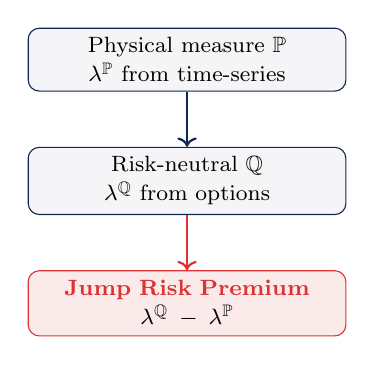
\begin{tikzpicture}[node distance=0.7cm and 1.2cm,
  mbox/.style={draw=darkblue,rounded corners,fill=lightgray,
              text width=3.8cm,align=center,font=\footnotesize}]
  \node[mbox] (P) {Physical measure $\mathbb{P}$\\[1pt]$\lambda^{\mathbb{P}}$ from time-series};
  \node[mbox, below=of P] (Q) {Risk-neutral $\mathbb{Q}$\\[1pt]$\lambda^{\mathbb{Q}}$ from options};
  \node[mbox, below=of Q,draw=accent,fill=accent!10] (JRP) {\textbf{\color{accent}Jump Risk Premium}\\[1pt]$\lambda^{\mathbb{Q}} - \lambda^{\mathbb{P}}$};
  \draw[->,thick,darkblue] (P) -- (Q);
  \draw[->,thick,accent]   (Q) -- (JRP);
\end{tikzpicture}
\end{block}

\column{0.52\textwidth}
\begin{block}{Current estimates ($\lambda^{\mathbb{P}}$)}
\footnotesize
\begin{itemize}\itemsep2pt
  \item Two-condition: $1.38$ / year (lower bound)
  \item Single-condition: $34$ / year (upper bound)
  \item Plausible structural range: \textbf{2--6} / year
\end{itemize}
\end{block}

\begin{alertblock}{W6 objective}
\footnotesize Calibrate Merton and Kou to QQQ option surface to recover $\lambda^{\mathbb{Q}}$.\\[2pt]
If $\lambda^{\mathbb{Q}} > \lambda^{\mathbb{P}}$: investors require compensation for bearing jump risk beyond pure expected value.
\end{alertblock}
\end{columns}
\end{frame}

\begin{frame}{Literature Arc \& Project Roadmap}
\begin{center}
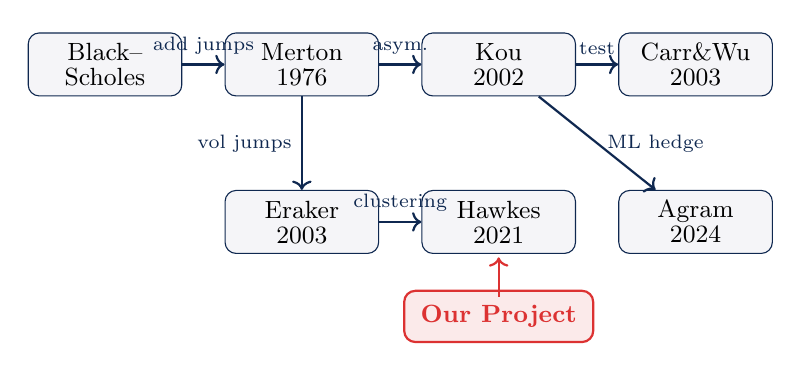
\begin{tikzpicture}[
  modelbox/.style={draw=darkblue,fill=lightgray,rounded corners,
               minimum width=1.95cm,minimum height=0.8cm,
               font=\small,align=center},
  arr/.style={->,thick,darkblue}]

  \node[modelbox] (BS) at (0,0)   {Black--\\[-2pt]Scholes};
  \node[modelbox] (M)  at (2.5,0) {Merton\\[-2pt]1976};
  \node[modelbox] (K)  at (5.0,0) {Kou\\[-2pt]2002};
  \node[modelbox] (CW) at (7.5,0) {Carr\&Wu\\[-2pt]2003};
  \node[modelbox] (E)  at (2.5,-2){Eraker\\[-2pt]2003};
  \node[modelbox] (H)  at (5.0,-2){Hawkes\\[-2pt]2021};
  \node[modelbox] (A)  at (7.5,-2){Agram\\[-2pt]2024};

  \draw[arr] (BS) -- (M)  node[midway,above,font=\scriptsize]{add jumps};
  \draw[arr] (M)  -- (K)  node[midway,above,font=\scriptsize]{asym.};
  \draw[arr] (K)  -- (CW) node[midway,above,font=\scriptsize]{test};
  \draw[arr] (M)  -- (E)  node[midway,left, font=\scriptsize]{vol jumps};
  \draw[arr] (E)  -- (H)  node[midway,above,font=\scriptsize]{clustering};
  \draw[arr] (K)  -- (A)  node[midway,right,font=\scriptsize]{ML hedge};

  \node[draw=accent,thick,rounded corners,fill=accent!10,
        minimum width=2.4cm,minimum height=0.65cm,
        font=\small\bfseries,text=accent] at (5.0,-3.2) {Our Project};
  \draw[->,thick,accent] (5.0,-2.95) -- (5.0,-2.45);
\end{tikzpicture}
\end{center}

\smallskip
\small\textbf{W1}: Lit.\ Review $\to$ \textbf{W2}: Math $\to$ \textbf{W3}: Monte Carlo $\to$ \textbf{W4}: COS $\to$ \textbf{W5}: Data \& jump detection $\to$ \textbf{W6}: Calibration \& risk premium
\end{frame}

\section{Conclusion}

\begin{frame}{Summary}
\begin{columns}[T]
\column{0.50\textwidth}
\begin{block}{What we showed}
\footnotesize
\begin{enumerate}\itemsep2pt
  \item B\&S fails: fat tails + volatility smile
  \item Merton (1976): Poisson jumps, closed-form pricing
  \item Kou (2002): asymmetric jumps, steeper skew
  \item Carr \& Wu (2003): jumps confirmed in index options
  \item Eraker et al.\ (2003): volatility jumps necessary
  \item Hawkes: jump clustering modelled endogenously
  \item Deep learning: LSTM hedges in incomplete markets
\end{enumerate}
\end{block}

\column{0.50\textwidth}
\begin{block}{Technical achievements}
\footnotesize
\begin{itemize}\itemsep2pt
  \item Monte Carlo with three variance-reduction methods
  \item COS engine: spectral convergence at $N=128$
  \item 732 days QQQ data; excess kurtosis $= 10.6$
  \item Jump detection: 4 confirmed, 99 candidate days
  \item Lognormal fit consistent with Merton ($p=0.12$)
\end{itemize}
\end{block}

\begin{alertblock}{Central finding}
\footnotesize Empirical QQQ kurtosis and option term structure are consistent with a combined jump-diffusion. The gap $\lambda^{\mathbb{Q}} - \lambda^{\mathbb{P}}$ is the jump risk premium to be estimated in W6.
\end{alertblock}
\end{columns}
\end{frame}

{
\setbeamertemplate{footline}{}
\begin{frame}[plain]
\begin{center}
  \vspace{1.8cm}
  {\Large\bfseries\color{darkblue} Thank You}\\[0.8cm]
  {\normalsize Merton Jump-Diffusion: Pricing and Harvesting\\
   the Equity Jump Risk Premium}\\[0.6cm]
  {\small Stochastic Processes --- Group 3 --- May 2026}
\end{center}
\end{frame}
}

\end{document}
